\documentclass[t,usenames,dvipsnames]{beamer}
\usetheme{Copenhagen}
\setbeamertemplate{headline}{} % remove toc from headers
\beamertemplatenavigationsymbolsempty

\usepackage{amsmath, sfmath, tikz, xcolor}
\usetikzlibrary{arrows.meta, calc}

\title{Dot Product and Projection}
\author{}
\date{}

\AtBeginSection[]
{
  \begin{frame}
    \frametitle{Table of Contents}
    \tableofcontents[currentsection]
  \end{frame}
}

\begin{document}

\begin{frame}
    \titlepage
\end{frame}

\section{Find the dot product of two vectors.}

\begin{frame}{Dot Product}
    For vectors $\vec{v} = \langle v_1, v_2 \rangle$ and $\vec{w} = \langle w_1, w_2 \rangle$, the \alert{dot product} of $\vec{v}$ and $\vec{w}$ is given as 
\begin{align*}
\vec{v} \cdot \vec{w} &= \langle v_1, v_2 \rangle \cdot \langle w_1, w_2 \rangle \\
\onslide<2->{&= v_1w_1 + v_2w_2}
\end{align*}
\end{frame}

\begin{frame}{Example 1}
Find $\vec{v} \cdot \vec{w}$ if $\vec{v} = \langle 3, 4 \rangle$ and $\vec{w} = \langle 1, -2 \rangle$.    
\begin{align*}
\onslide<2->{\vec{v}\cdot\vec{w} &= \langle 3, 4\rangle \cdot \langle 1, -2\rangle} \\[8pt]
\onslide<3->{&= 3(1) + 4(-2)} \\[8pt]
\onslide<4->{&= -5} \\
\end{align*}
\end{frame}

\begin{frame}{Dot Product Properties}
Because the dot product produces a scalar, it is often called the \alert{scalar product}.    \newline\\

\onslide<2->{\textbf{Properties}} \newline\\
\begin{tabular}{ll}
    \onslide<3->{$\vec{v} \cdot \vec{w} = \vec{w} \cdot \vec{v}$ &
    Commutative Property}    \\[8pt]
    \onslide<4->{$\vec{u} \cdot \left(\vec{v} + \vec{w}\right) = \vec{u} \cdot \vec{v} + \vec{u} \cdot \vec{w}$  &   Distributive Property} \\[8pt]
    \onslide<5->{$k\left(\vec{v}\right) \cdot \vec{w} = k\left(\vec{v} \cdot \vec{w}\right) = \vec{v} \cdot \left(k\vec{w}\right)$    &   Scalar Property}    \\[8pt]
    \onslide<6->{$\vec{v} \cdot \vec{v} = \lVert \vec{v} \rVert ^2$  &
    Relation to Magnitude} \\[8pt]
\end{tabular}
\end{frame}

\begin{frame}{Example 2}
    Show that $ \lVert \vec{v} - \vec{w} \rVert ^2 = \lVert \vec{v} \rVert ^2 - 2\left( \vec{v} \cdot \vec{w} \right) + \lVert \vec{w} \rVert ^2 $
\begin{align*}
    \onslide<2->{\lVert \vec{v} - \vec{w} \rVert &= (\vec{v} - \vec{w})\cdot (\vec{v} - \vec{w})} \\[8pt]
    \onslide<3->{&= \vec{v}\cdot(\vec{v}-\vec{w}) -\vec{w} \cdot (\vec{v}-\vec{w})} \\[8pt]
    \onslide<4->{&=\vec{v}\cdot\vec{v} - \vec{v}\cdot\vec{w} - \vec{v}\cdot\vec{w} + \vec{w}\cdot\vec{w}} \\[8pt]
    \onslide<5->{&= \vec{v}\cdot\vec{v} - 2(\vec{v}\cdot\vec{w}) + \vec{w}\cdot\vec{w}} \\[8pt]
    \onslide<6->{&= \lVert v\rVert^2 - 2(\vec{v}\cdot\vec{w}) + \lVert w \rVert^2} \\
\end{align*}
\end{frame}

\section{Find the angle measure between two vectors.}

\begin{frame}{Angles Between Vectors}
    If we draw $\vec{v}$ and $\vec{w}$ with the same initial point, then the angle $\theta$ between them is illustrated below:  \newline\\

\begin{tabular}{p{0.3\textwidth}p{0.3\textwidth}p{0.25\textwidth}}
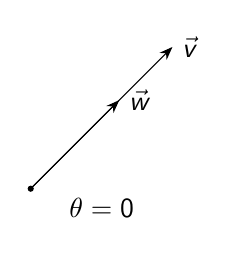
\begin{tikzpicture}[scale=0.9]
    \draw [-{Stealth}] (0,0) -- (2,2) node [right] {$\vec{v}$};
    \draw [-{Stealth}] (0,0) -- (1.25,1.25) node [right] {$\vec{w}$};
    \draw [fill=black] (0,0) circle (1pt);
    \node at (1,0) [below] {$\theta = 0$};
\end{tikzpicture}
&
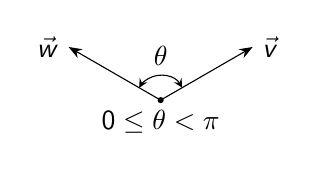
\begin{tikzpicture}[scale=0.9]
    \draw [-{Stealth}] (0,0) -- (30:1.5) node [right] {$\vec{v}$};
    \draw [-{Stealth}] (0,0) -- (150:1.5) node [left] {$\vec{w}$};
    \draw [fill=black] (0,0) circle (1pt);
    \draw [<->, >=stealth] (30:0.35) arc (30:150:0.35) node [midway, above] {$\theta$};
    \node at (0,0) [below] {$0 \leq \theta < \pi$};
\end{tikzpicture}
&
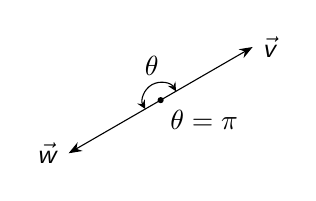
\begin{tikzpicture}[scale=0.9]
    \draw [-{Stealth}] (0,0) -- (30:1.5) node [right] {$\vec{v}$};
    \draw [-{Stealth}] (0,0) -- (210:1.5) node [left] {$\vec{w}$};
    \draw [fill=black] (0,0) circle (1pt);
    \draw [<->, >=stealth] (30:0.25) arc (30:210:0.25) node [midway, above] {$\theta$};
    \node at (0,0) [below right] {$\theta = \pi$};
\end{tikzpicture}   
\end{tabular}
\end{frame}

\begin{frame}{Dot Product and Angles Between Vectors}
Geometrically, the dot product between two vectors is 
\[
\vec{v} \cdot \vec{w} = \lVert \vec{v} \rVert \lVert \vec{w} \rVert \cos \theta
\]
\vspace{20pt}
\pause
\begin{tabular}{p{0.5\textwidth}p{0.35\textwidth}}
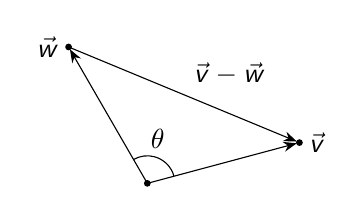
\begin{tikzpicture}
    \draw [-{Stealth}, shorten >= 1pt] (0,0) -- (15:2) node [right] {$\vec{v}$};
    \draw [-{Stealth}, shorten >= 1pt] (0,0) -- (120:2) node [left] {$\vec{w}$};
    \draw [-{Stealth}, shorten >= 1pt] (120:2) -- (15:2) node [midway, above right] {$\vec{v}-\vec{w}$};
    \draw (15:0.35) arc (15:120:0.35) node [midway, above] {$\theta$};
    \draw [fill=black] (15:2) circle (1pt);
    \draw [fill=black] (120:2) circle (1pt);
    \draw [fill=black] (0,0) circle (1pt);
\end{tikzpicture}
&
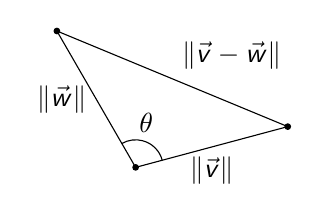
\begin{tikzpicture}
    \draw (0,0) -- (15:2) node [midway, below] {$\lVert \vec{v} \rVert$};
    \draw (0,0) -- (120:2) node [midway, left] {$\lVert \vec{w} \rVert$};
    \draw (120:2) -- (15:2) node [midway, above right] {$\lVert \vec{v}-\vec{w} \rVert$};
    \draw (15:0.35) arc (15:120:0.35) node [midway, above] {$\theta$};
    \draw [fill=black] (15:2) circle (1pt);
    \draw [fill=black] (120:2) circle (1pt);
    \draw [fill=black] (0,0) circle (1pt);
\end{tikzpicture}   \\[8pt]
\end{tabular}    
\end{frame}

\begin{frame}{Dot Product and Angles Between Vectors}
By the Law of Cosines, $\lVert \vec{v} - \vec{w} \rVert ^2 = \lVert \vec{v} \rVert ^2 + \lVert \vec{w} \rVert ^2 - 2 \lVert \vec{v} \rVert \lVert \vec{w} \rVert \cos \theta$, and by Example 2, $ \lVert \vec{v} - \vec{w} \rVert ^2  = \lVert \vec{v} \rVert ^2 - 2\left( \vec{v} \cdot \vec{w} \right) + \lVert \vec{w} \rVert ^2 $.    \\[11pt]
\pause
Equating these and solving for $\vec{v} \cdot \vec{w}$ gives us $\vec{v} \cdot \vec{w} = \lVert \vec{v} \rVert \lVert \vec{w} \rVert \cos \theta$, from which
\[
\cos \theta = \frac{\vec{v} \cdot \vec{w}}{\lVert \vec{v} \rVert \, \lVert \vec{w} \rVert}
\]
\pause
\vspace{11pt}
To find the angle between two vectors, solve for $\theta$:
\[
\theta = \cos^{-1}\left(\frac{\vec{v} \cdot \vec{w}}{\lVert \vec{v} \rVert \, \lVert \vec{w} \rVert} \right) = \cos^{-1}\left(\hat{v} \cdot \hat{w} \right)
\]
\end{frame}

\begin{frame}{Example 3a}
Find the angle between each of the following.   \newline\\
(a) \quad $\vec{v} = \langle 3, -3\sqrt{3} \rangle$ and $\vec{w} = \langle -\sqrt{3}, 1 \rangle$
\begin{align*}
    \onslide<2->{\vec{v}\cdot\vec{w} &= \langle 3, -3\sqrt{3} \rangle \cdot \langle -\sqrt{3}, 1 \rangle} \\[8pt]
    \onslide<3->{&= -3\sqrt{3}-3\sqrt{3}=-6\sqrt{3}} \\[8pt]
    \onslide<4->{\lVert \vec{v} \rVert &= \sqrt{3^2 + (3\sqrt{3})^2} = \sqrt{36}} \\[8pt]
    \onslide<5->{\lVert \vec{w} \rVert &= \sqrt{(\sqrt{3})^2 + 1^2} = \sqrt{4}} \\[8pt]
    \onslide<6->{\theta &= \arccos\left(\frac{-6\sqrt{3}}{\sqrt{36\times 4}}\right) = \frac{5\pi}{6}} 
\end{align*}
\end{frame}

\begin{frame}{Example 3b}
(b) \quad $\vec{v} = \langle 2, 2 \rangle$ and $\vec{w} = \langle 5, -5 \rangle$
\begin{align*}
    \onslide<2->{\vec{v}\cdot\vec{w} &= 2(5) + 2(-5) = 0} \\[8pt]
    \onslide<3->{\lVert \vec{v} \rVert &= \sqrt{2^2 + 2^2} = \sqrt{8}} \\[8pt]
    \onslide<4->{\lVert \vec{w} \rVert &= \sqrt{5^2 + 5^2} = \sqrt{50}} \\[8pt]
    \onslide<5->{\theta &= \arccos\left(\frac{0}{\sqrt{8\times50}}\right) = \frac{\pi}{2}} \\
\end{align*}
\end{frame}

\begin{frame}{Example 3c}
(c) \quad  $\vec{v} = \langle 3, -4 \rangle$ and $\vec{w} = \langle 2, 1 \rangle$
\begin{align*}
    \onslide<2->{\vec{v}\cdot\vec{w} &= 3(2) + (-4)(1) = 2} \\[8pt]
    \onslide<3->{\lVert \vec{v} \rVert &= \sqrt{3^2+4^2} = \sqrt{25}} \\[8pt]
    \onslide<4->{\lVert \vec{w} \rVert &= \sqrt{2^2 + 1^2} = \sqrt{5}} \\[8pt]
    \onslide<5->{\theta &= \arccos{\left(\frac{2}{\sqrt{25\times5}}\right)} \approx 80^\circ}
\end{align*}
\end{frame}

\section{Find the projection of one vector onto another.}

\begin{frame}{Orthogonal Projection}
Two vectors are {\color{blue}\textbf{orthogonal}} if they meet at a right angle.  \newline\\

If two vectors are orthogonal, then their dot product is 0.  
\end{frame}

\begin{frame}{Orthogonal Projection}
The \alert{orthogonal projection} of $\vec{v}$ onto $\vec{w}$ is a new vector $\vec{p}$ that is parallel to $\vec{w}$ and has a magnitude of $\lVert \vec{v} \rVert \cos \theta$.    \newline\\ \pause

$\vec{p}$ can be thought of as the ``shadow" $\vec{v}$ casts over $\vec{w}$: \newline\\

\begin{tabular}{p{0.4\textwidth}p{0.25\textwidth}}
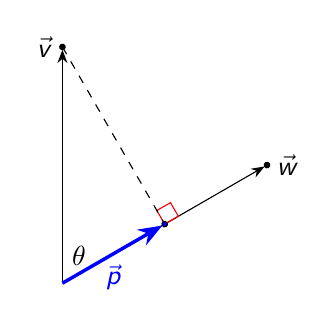
\begin{tikzpicture}[rotate=30]
    \coordinate (A) at (0:3);
    \coordinate (B) at (60:3);
    \draw [-{Stealth}, shorten >= 1pt] (0,0) -- (A) node [right] {$\vec{w}$};
    \draw [fill = black] (A) circle (1pt);
    \draw [-{Stealth}, shorten >= 1pt] (0,0) -- (B) node [left] {$\vec{v}$};
    \draw [fill = black] (B) circle (1pt);
    \draw [color=red] (1.5,0) rectangle +(0.2,0.2);
    \draw [dashed] (B) -- (1.5,0);
    \node at (0,0) [above right, yshift = 0.1cm] {$\theta$};
    \draw [-{Stealth}, line width = 1.25, color = blue, shorten >= 1pt] (0,0) -- (1.5,0) node [midway, below] {$\vec{p}$};
    \draw [fill=blue] (1.5,0) circle (1pt);
\end{tikzpicture}
&
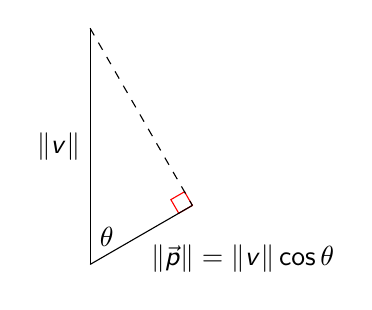
\begin{tikzpicture}[rotate=30]
    \coordinate (B) at (60:3);
    \draw  (0,0) -- (B) node [midway, left] {$\lVert v \rVert$};
    \draw [color=red] (1.5,0) rectangle +(-0.2,0.2);
    \draw [dashed] (B) -- (1.5,0);
    \node at (0,0) [above right, yshift = 0.1cm] {$\theta$};
    \draw (0,0) -- (1.5,0) node [midway, below right] {$\lVert \vec{p} \rVert = \lVert v \rVert \cos \theta$};
\end{tikzpicture}   \\[8pt]
\end{tabular}    
\end{frame}

\begin{frame}{Orthogonal Projection}
We need $\vec{p}$ to be parallel to $\vec{w}$. To do this, we could take the dot product of $\vec{p}$ and $\vec{w}$. \newline\\
\pause
However, that would likely change the magnitude of $\vec{p}$. \newline\\
\pause
Recall that when finding a unit vector for a given vector, that unit vector has a magnitude of 1 and is parallel to the original vector.  \newline\\
\pause

Thus, we can multiply the magnitude of $\vec{p}$ by a unit vector for $\vec{w}$.
\[
    \lVert \vec{p} \rVert \, \hat{w}
\]
\pause
This will guarantee that $\vec{w}$ is scaled to $\vec{p}$ and give us the projection of $\vec{v}$ onto $\vec{w}$.
\end{frame}

\begin{frame}{Orthogonal Projection}
\begin{minipage}{0.4\textwidth}
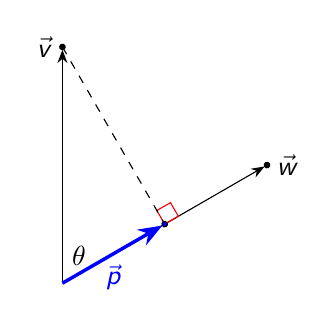
\begin{tikzpicture}[rotate=30]
    \coordinate (A) at (0:3);
    \coordinate (B) at (60:3);
    \draw [-{Stealth}, shorten >= 1pt] (0,0) -- (A) node [right] {$\vec{w}$};
    \draw [fill = black] (A) circle (1pt);
    \draw [-{Stealth}, shorten >= 1pt] (0,0) -- (B) node [left] {$\vec{v}$};
    \draw [fill = black] (B) circle (1pt);
    \draw [color=red] (1.5,0) rectangle +(0.2,0.2);
    \draw [dashed] (B) -- (1.5,0);
    \node at (0,0) [above right, yshift = 0.1cm] {$\theta$};
    \draw [-{Stealth}, line width = 1.25, color = blue, shorten >= 1pt] (0,0) -- (1.5,0) node [midway, below] {$\vec{p}$};
    \draw [fill=blue] (1.5,0) circle (1pt);
\end{tikzpicture}
\end{minipage}
\begin{minipage}{0.5\textwidth}
\begin{align*}
\onslide<2->{\text{proj}_{\vec{w}} \vec{v} &= \lVert {\color{blue}{\vec{p}}} \rVert \, {\color{red}\hat{w} }} \\[8pt]
%%%%%%%%%%%%%%%%%%%%%%%%%%%%%%%%%%%%%%%%%%%%%%%%%%%
\onslide<3->{&= \left( {\color{blue}{\lVert v \rVert \cos \theta }}\right) \left( {\color{red}\frac{\vec{w}}{\lVert w \rVert} } \right)} \\[8pt]
%%%%%%%%%%%%%%%%%%%%%%%%%%%%%%%%%%%%%%%%%%%%%%%%%%%
\onslide<4->{&= \lVert {\color{blue}v} \rVert \left( {\color{blue}\frac{v \cdot w}{\lVert v \rVert \, \lVert w \rVert} } \right) \left({\color{red}\frac{\vec{w}}{\lVert w \rVert} } \right)} \\[8pt]
%%%%%%%%%%%%%%%%%%%%%%%%%%%%%%%%%%%%%%%%%%%%%%%%%%%
\onslide<5->{&= \left({\color{blue}\frac{v \cdot w}{\lVert w \rVert \, {\color{red}\lVert w \rVert}} } \right) {\color{red}\vec{w} } }  \\[8pt]
%%%%%%%%%%%%%%%%%%%%%%%%%%%%%%%%%%%%%%%%%%%%%%%%%%%
\onslide<6->{\text{proj}_{\vec{w}} \vec{v} &= \left({\color{blue} \frac{v \cdot w}{\lVert w \rVert ^2} } \right) {\color{red}\vec{w} }}
\end{align*}
\end{minipage}
\end{frame}

\begin{frame}{Example 4a}
Let $\vec{v} = \langle 1, 8 \rangle$ and $\vec{w} = \langle -1, 2 \rangle$. Find each of the following.   \newline\\
(a) \quad $\text{proj}_{\vec{w}} \vec{v}$
\begin{align*}
    \onslide<2->{\text{proj}_{\vec{w}} \vec{v} &= \left(\frac{v \cdot w}{\lVert w \rVert^2}\right)\vec{w}} \\[8pt]
    \onslide<3->{v \cdot w = 1(-1) + 8(2) = 15} \quad & \quad \onslide<4->{\lVert \vec{w} \rVert^2 = \left(\sqrt{1^2+2^2}\right)^2 = 5} \\[8pt]
    \onslide<5->{\text{proj}_{\vec{w}} \vec{v} &= \frac{15}{5}\left<-1, 2\right>} \\[8pt]
    \onslide<6->{&= 3\langle -1, 2\rangle} \\[8pt]
    \onslide<7->{&= \langle -3, 6\rangle} \\
\end{align*}
\end{frame}

\begin{frame}{Example 4b}
Let $\vec{v} = \langle 1, 8 \rangle$ and $\vec{w} = \langle -1, 2 \rangle$. Find each of the following.   \newline\\
(b) \quad   $\text{proj}_{\vec{v}} \vec{w}$
\begin{align*}
\onslide<2->{\text{proj}_{\vec{v}} \vec{w} &= \left(\frac{w \cdot v}{\lVert v \rVert^2}\right)\vec{v}} \\[8pt]
    \onslide<3->{w \cdot v = 1(-1) + 8(2) = 15} \quad & \quad \onslide<4->{\lVert \vec{v} \rVert^2 = \left(\sqrt{1^2+8^2}\right)^2 = 65} \\[8pt]
    \onslide<5->{\text{proj}_{\vec{v}} \vec{w} &= \frac{3}{13}\left<1, 8\right>} \\[8pt]
    \onslide<6->{&= \left< \frac{3}{13}, \frac{24}{13}\right>} \\[8pt]    
\end{align*}
\end{frame}

\section{Find the work done in applying a force to an object.}

\begin{frame}{Work}
    In physics, if a constant force $F$ is exerted over a distance (really, \textit{displacement}) $d$, the work $W$ done by the force is given by $W=Fd$.  \newline\\
\pause
However, if the force being applied is not in the direction of motion, we can use the dot product to find the work done. \newline\\
\pause
\begin{center}
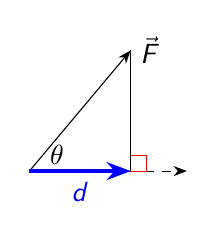
\begin{tikzpicture}
    \coordinate (O) at (0,0);
    \coordinate (F) at (50:2);
    \coordinate (A) at (2,0);
    \draw [-{Stealth}, dashed] (O) -- (A);
    \draw [-{Stealth}] (O) -- (F) node [right] {$\vec{F}$};
    \draw [color=red] ($(O)!(F)!(A)$) rectangle +(0.2,0.2);
    \draw ($(O)!(F)!(A)$) -- (F);
    \draw [-{Stealth}, line width = 1.25, color=blue] (O) -- ($(O)!(F)!(A)$) node [midway, below] {\color{blue}$d$};
    \node at (O) [yshift=0.2cm, xshift=0.35cm] {$\theta$};
\end{tikzpicture}

$W = Fd = \lVert F \rVert \, \lVert d \rVert \cos \theta = F \cdot d$
\end{center}
\end{frame}

\begin{frame}{Example 5}
Mr. Bain exerts a force of 230 pounds to pull a stack of rocks a distance of 50 ft. over level ground. If the rope makes a $30^\circ$ angle with the horizontal, how much work did Mr. Bain do pulling the rocks? Assume Mr. Bain exerts the force of 230 pounds at a $30^\circ$ angle for the duration of the 50 feet.  
\begin{align*}
    \onslide<2->{W &= \lVert F\rVert \lVert d \rVert \cos\theta} \\[8pt]
    \onslide<3->{&= (230\text{ pounds})(50\text{ ft})\cos30^\circ} \\[8pt]
    \onslide<4->{&= 11,500\text{ foot-pounds}\left(\frac{\sqrt{3}}{2}\right)} \\[8pt]
    \onslide<5->{&= 5,750\sqrt{3}\,(\approx 9,959.3)\text{ foot-pounds}} \\
\end{align*}
\end{frame}


\end{document}
